\chapter{\babTiga}
Perancangan serta langkah-langkah di perlukan untuk menyelesaikan penelitian ini. Berikut ini akan di jelaskan gambaran serta tahapan dari perancangan system yang di teliti serta skenario simulasi dari hasil desain yang telah dirancang.

\section{Desain}
Secara garis besar pada sisi desainer, terdapat 3 langkah untuk melakukan pengembangan alat dari programming hingga layout siap cetak. Penulis menggunakan cara ini dari hasil studi serta eksperimen saat proses pengembangan alat.

\begin{figure}
	\centering
	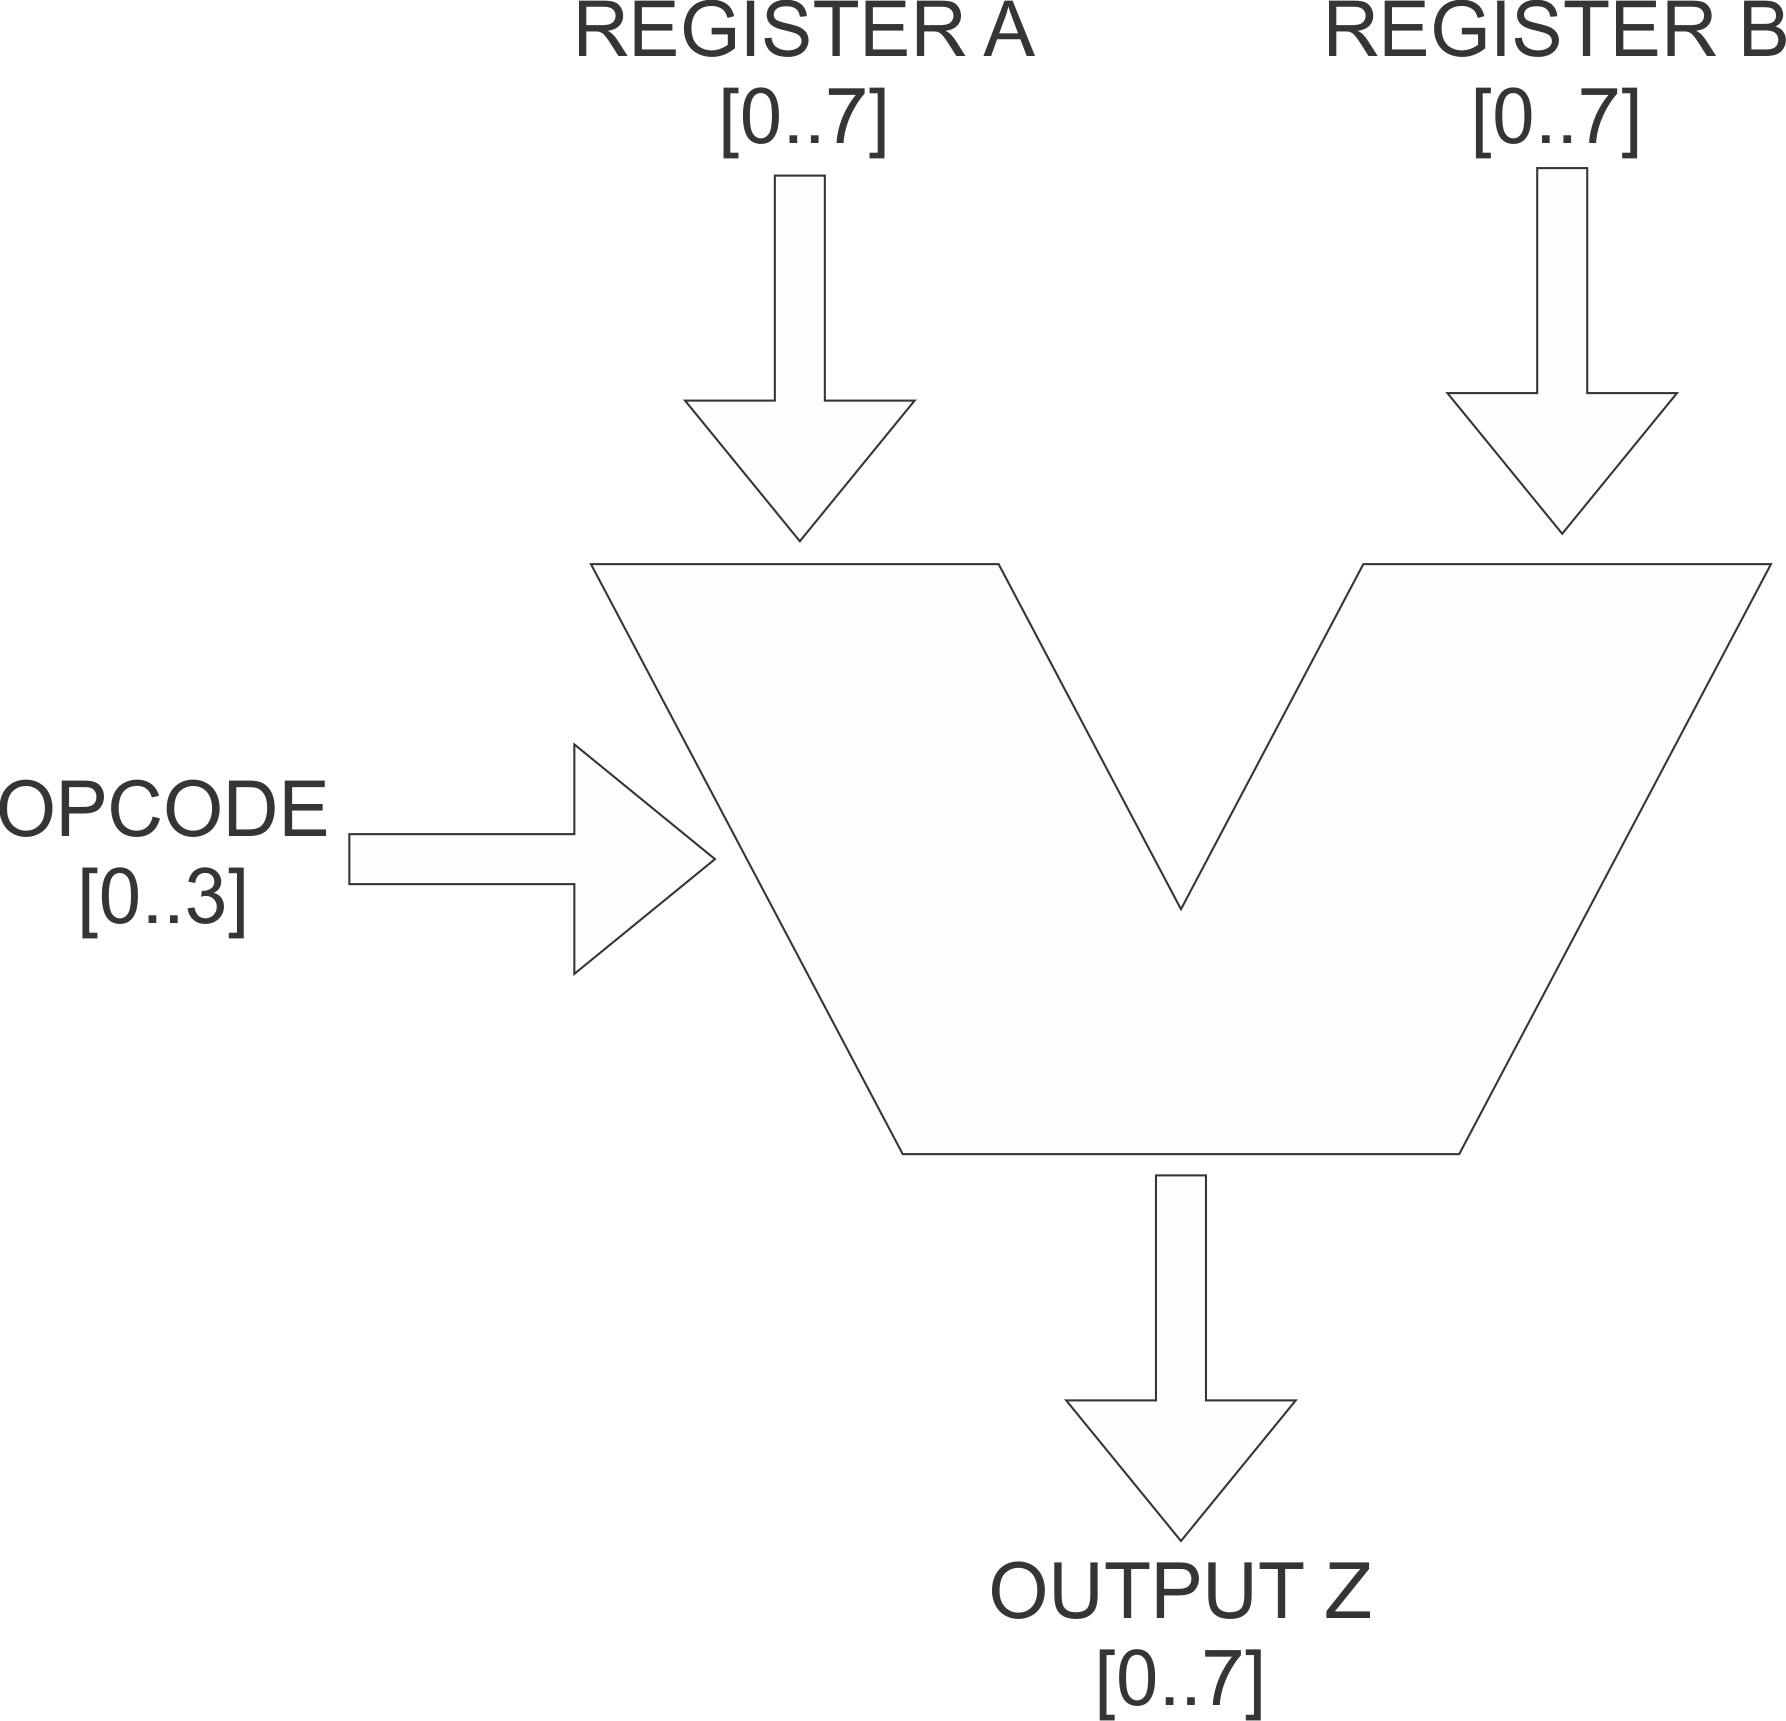
\includegraphics[width=0.5\textwidth]
	{ilustrasi/aludesain.png}
	\caption{Desain ALU yang akan dilindungi}
	\label{aludesain}
\end{figure}

\begin{figure}
	\centering
	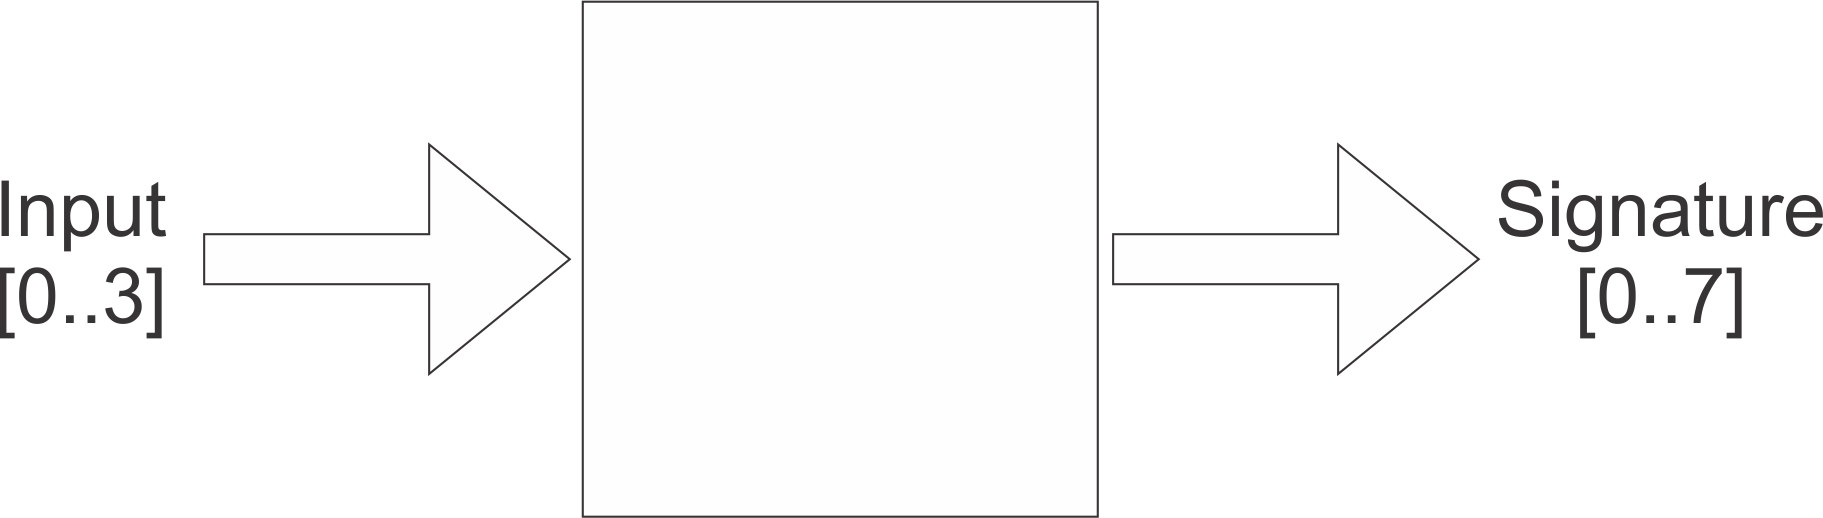
\includegraphics[width=0.5\textwidth]
	{ilustrasi/watermarkdesain.png}
	\caption{Desain rangkaian pelindung}
	\label{watermarkdesain}
\end{figure}

\subsection{Skema Perlindungan}

\begin{figure}
	\centering
	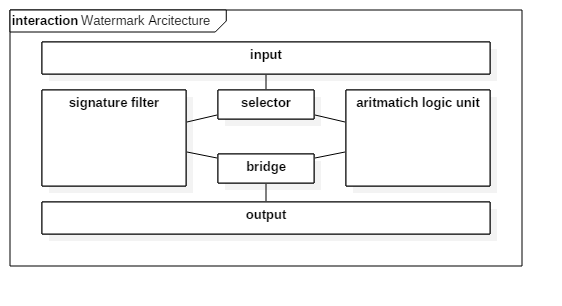
\includegraphics[width=1.0\textwidth]
	{diagrams/watermark_arcitechture.png}
	\caption{Arsitektur watermark}
	\label{fig:arsitektur}
\end{figure}

\begin{figure}
	\centering
	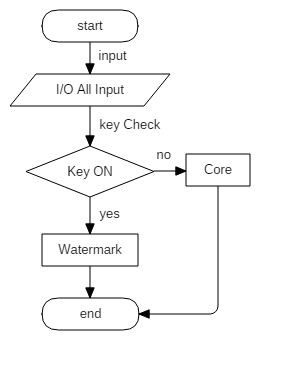
\includegraphics[width=0.5\textwidth]
	{diagrams/Activation.png}
	\caption{Aktifasi}
	\label{fig:aktifasi}
\end{figure}

\begin{figure}
	\centering
	\includegraphics[width=1.0\textwidth]
	{diagrams/watermark_arcitecture_off.png}
	\caption{Arsitektur watermark off}
	\label{fig:arsitekturoff}
\end{figure}

\begin{figure}
	\centering
	\includegraphics[width=1.0\textwidth]
	{diagrams/watermark_arcitecture_on.png}
	\caption{Arsitektur watermark on}
	\label{fig:arsitekturon}
\end{figure}

\subsection{Spesifikasi}
\todo{isi sendiri}

\section{Alur Proses Pengembangan}

\begin{figure}
	\centering
	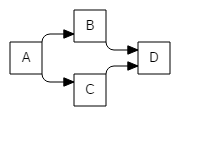
\includegraphics[width=0.3\textwidth]
	{diagrams/All_General.png}
	\caption{Skema Perancangan Umum Proses Desain}
	\label{fig:Allgeneral}
\end{figure}

Pada langkah pertama dilakukan proses A, penulis melakukan perancangan desain dari IC yang akan di watermark kemudian di lakukan analisis. Apabila pertama telah selesai, penulis akan melakukan langkah kedua. Pada langkah kedua ini di lakukan kegiatan B yaitu proses ferifikasi dengan FPGA dan kegiatan C yaitu proses syntesys menjadi Raw Layout. Setelah kegiatan B dan C selesai maka kegiatan D yaitu proses finalisasi layout dapat dilakukan yang akhirnya hasil final layout dapat di serahkan ke pabrik untuk di fabrikasi.

\begin{figure}
	\centering
	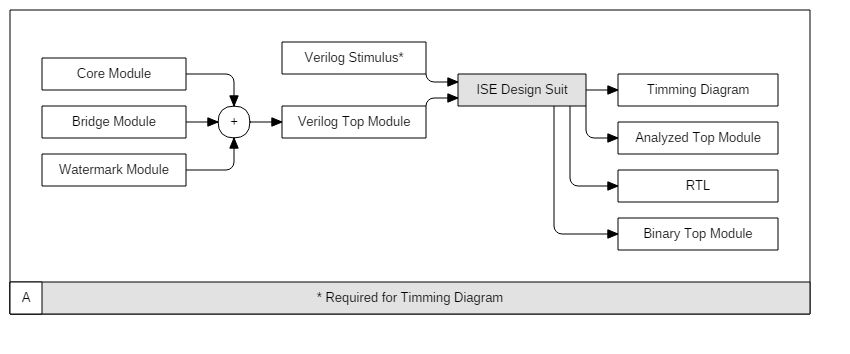
\includegraphics[width=1.0\textwidth]
	{diagrams/kegiatanA.png}
	\caption{Skema Perancangan dari Sub Proses Desain}
	\label{kegiatanA}
\end{figure}

Secara umum pada kegiatan A, penulis membuat 3 module verilog untuk digabungkan. Core Module yaitu program rangkaian ALU, Watermark Module adalah program untuk watermarking dan Bridge Module untuk menghubungkan output antara Core Module dan Watermark Module. Setelah selesai dilakukan programming setiap medule tersebut maka medul-modul tadi digabungkan menjadi Top Module. Top Module ini lah yang nantinya akan menjadi IC terwatermark. 

Pada top module ini harus diberikan program tambahan yaitu stimulus untuk dapat mensimulasikan skenario Input dan Output dari Top Module. Bila sekenario stimulus telah dibuat, kemudian dilakukan simulasi dengan bantuan softwere ISE design suit untuk melihat hasil simulasi berupa Timming diagram. Pada Timming Diagram inilah dapat di lihat apakah sekenario dari Input dan Output sesuai dengan keinginan. Setelah hasil analisis sesuai dengan yang diinginkan maka dilanjutkan dengan kegiatan selanjutnya yaitu kegiatan B dan C.

\begin{figure}
	\centering
	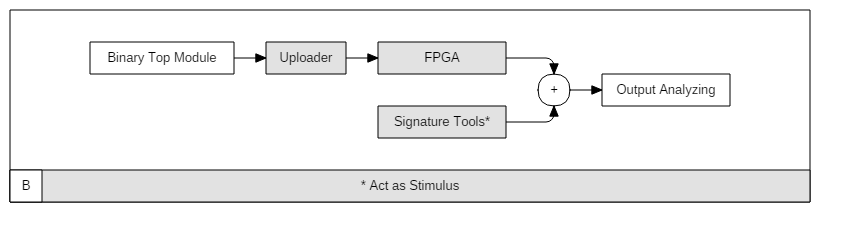
\includegraphics[width=1.0\textwidth]
	{diagrams/kegiatanB.png}
	\caption{Skema Perancangan dari Sub Proses Desain}
	\label{kegiatanB}
\end{figure}

Pada kegiatan B ini dilakukan simulasi ferivikasi pada board FPGA dengan alat ferifikasi. kegiatan ini dilakukan untuk simulasi ferifikasi signature pada IC yang telah diwatermark. IC yang telah diwatermak di tanam pada FPGA dan dengan menggunakan Signature Tools dilakukan ferifikasi sehingga didapat data signature dari IC yang telah di watermask.

\begin{figure}
	\centering
	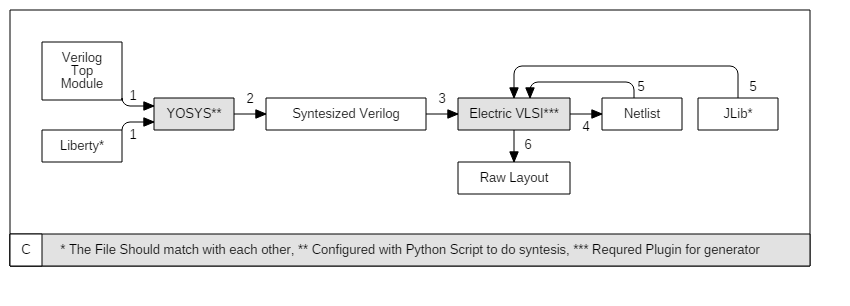
\includegraphics[width=1.0\textwidth]
	{diagrams/kegiatanC.png}
	\caption{Skema Perancangan dari Sub Proses Desain}
	\label{kegiatanC}
\end{figure}

Untuk kegiatan C dilakukan developing layout dari Top Module yang telah diferifikasi dengan timming diagram. Defeloping menggunakan softwere Electric VLSI. Dengan mensyntesis Verilog Top Module dan Liberty file menggunakan YOSYS, maka akan di dapat file verilog tersyntesis. Kemudian File tersintesis tersebut di Load di Electric VLSI untuk di rubah ke NetList. Setelah berhasil di rubah menjadi NetList maka file NetList tersebut di kompilasi bersama file JLib pada electric VLSI untuk di jadikan Raw Layout.

\begin{figure}
	\centering
	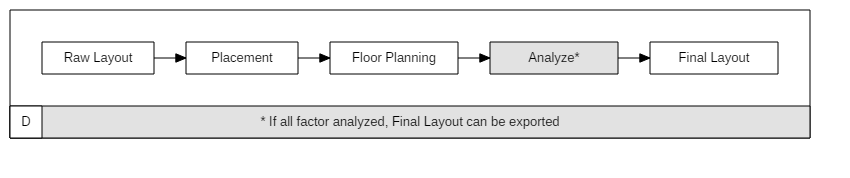
\includegraphics[width=1.0\textwidth]
	{diagrams/kegiatanD.png}
	\caption{Skema Perancangan dari Sub Proses Desain}
	\label{kegiatanD}
\end{figure}

Pada tahap ini di lakukan kegiatan C yaitu memproses Raw Layout menjadi Final Layout yang siap di cetak. Tahapan nya adalah melakukan placement untuk setiap modulnya lalu di lakukan analisis kemudian dilakukan Floor planning. Setelah itu dilakukan analisis kembali hingga didapat hasil yang terbaik. Apabila telah didapat hasil yang terbaik maka File siap untuk difabrikasi.

\section{Simulasi}
\todo{jelasin dan tampilin simulasi apa aja yang bakal gw lakuin disini}
